\documentclass[letterpaper, 12pt]{artikel3}

\usepackage{geometry}
\geometry{left=3cm,right=3cm,top=4cm,bottom=4cm}
\usepackage[fleqn]{amsmath}

% These packages add a few useful math symbols.
\usepackage{amssymb}
\usepackage{amsmath}
\usepackage{mathtools}
\usepackage{listings}
\usepackage{amsmath}
\usepackage{amssymb}
\lstset{language=Matlab}
\usepackage{euler}


%Karnaugh map
\usepackage{tikz}
\usepackage{askmaps}
\usepackage{circuitikz}
\usetikzlibrary{matrix,calc}
\usetikzlibrary{automata,positioning}
\usepackage{amssymb}
\usepackage{tikz}


\usetikzlibrary{circuits.logic.US,circuits.logic.IEC}

% The verbatim package allows pre-formatted text (like code) to be included.
\usepackage{verbatim}

% The algorithmic package provides a somewhat convenient way to typeset
% algorithms.
\usepackage{algorithm}
\usepackage[noend]{algpseudocode}

\usepackage{float}

\makeatletter
\def\BState{\State\hskip-\ALG@thistlm}
\makeatother

\usepackage{fancyhdr}
\pagestyle{fancy}
\lhead{}
\chead{CSC421 Artificial Intelligence  Assignment \#4 | YUE LYU V00902738}
\rhead{}
\renewcommand{\headrulewidth}{0.4pt}

\begin{document}

\section*{Question HMM Question}
\subsection*{a}
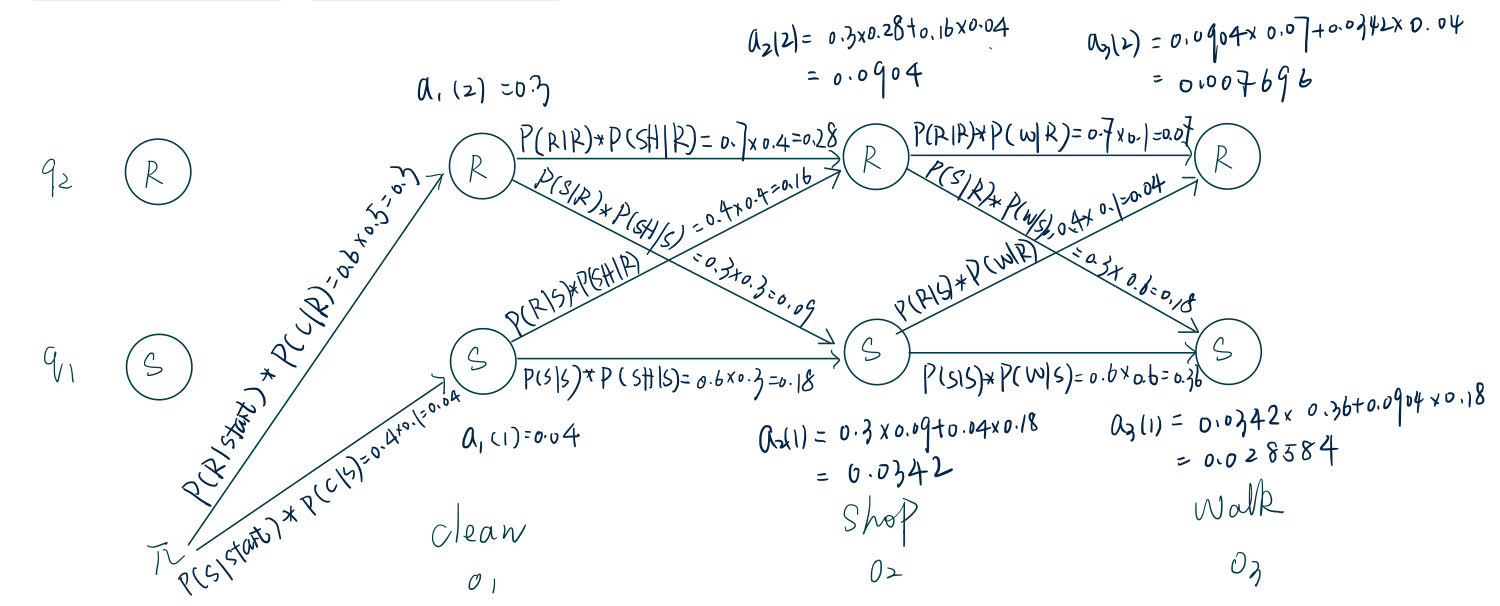
\includegraphics[scale=0.3]{a1.jpg}
P(Clean, Shop, Walk) = 0.007696+0.028584 = 0.03628
\subsection*{b}
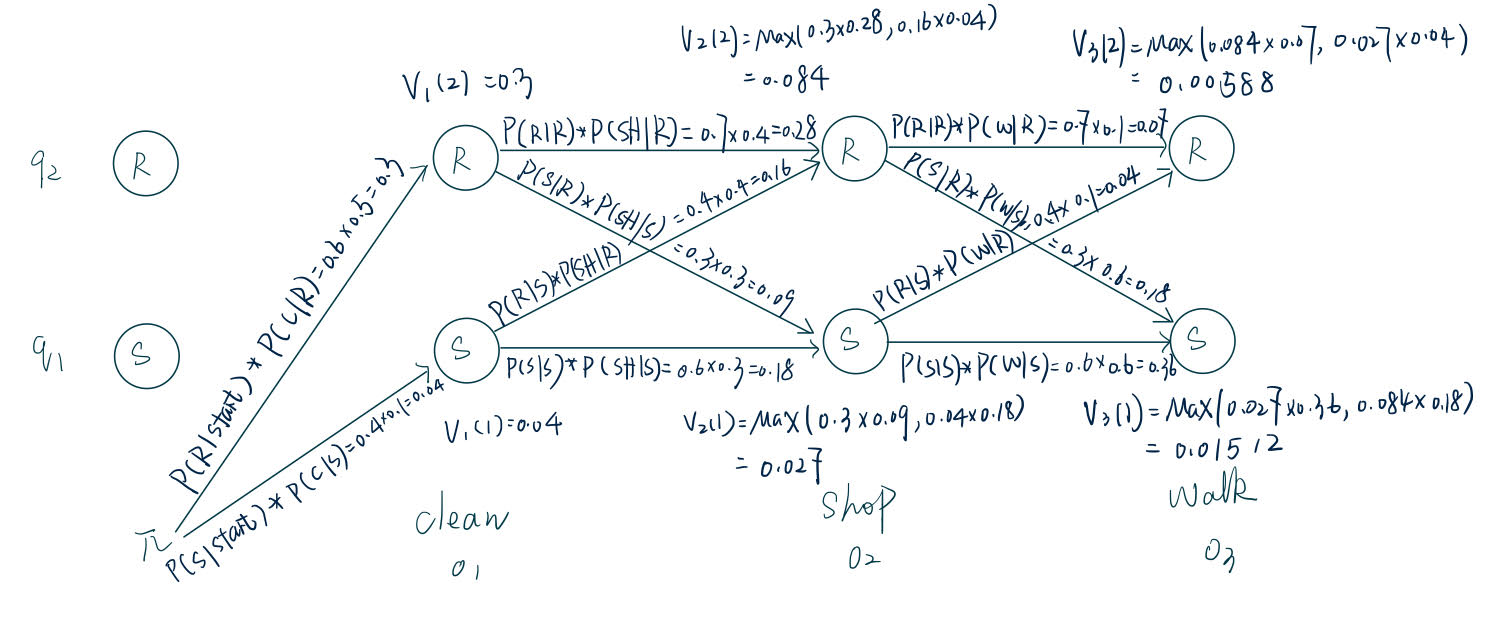
\includegraphics[scale=0.3]{a2.jpg}
Most likely sequence of hidden states: Rainy, Rainy, Sunny
\end{document}
